\chapter{Europe rail networks - Task 45}

A comprehensive dataset of European railroads (2019) from \href{https://www.mapsforeurope.org/datasets/euro-global-map}{EuroGlobalMap} is analyzed. 
The dataset consists of two objects: linestrings\footnote{Linestring objects are a series of points (each with its own coordinate) connected successively with each other.} and points, the former represent rail roads, while the latter are train stations. 
The resulting graph consists of two kind of nodes, station ($s$) and non-station ($ns$) nodes.\\
Although the fine details can be very important, the first instinct was to use the $ns$ nodes to build a network consisting entirely of $s$ nodes, connected if a path that does not cross any other $s$ node exists between them. However, this task is extremely challenging while keeping an undirected graph with no additional node-metadata, the fundamental reason is because of rail junctions.

\begin{wrapfigure}{r}{7.5cm}  
\label{fig: junctionexample}
  \centering
  \vspace{-\baselineskip}    % (optional) nudge upward a bit
  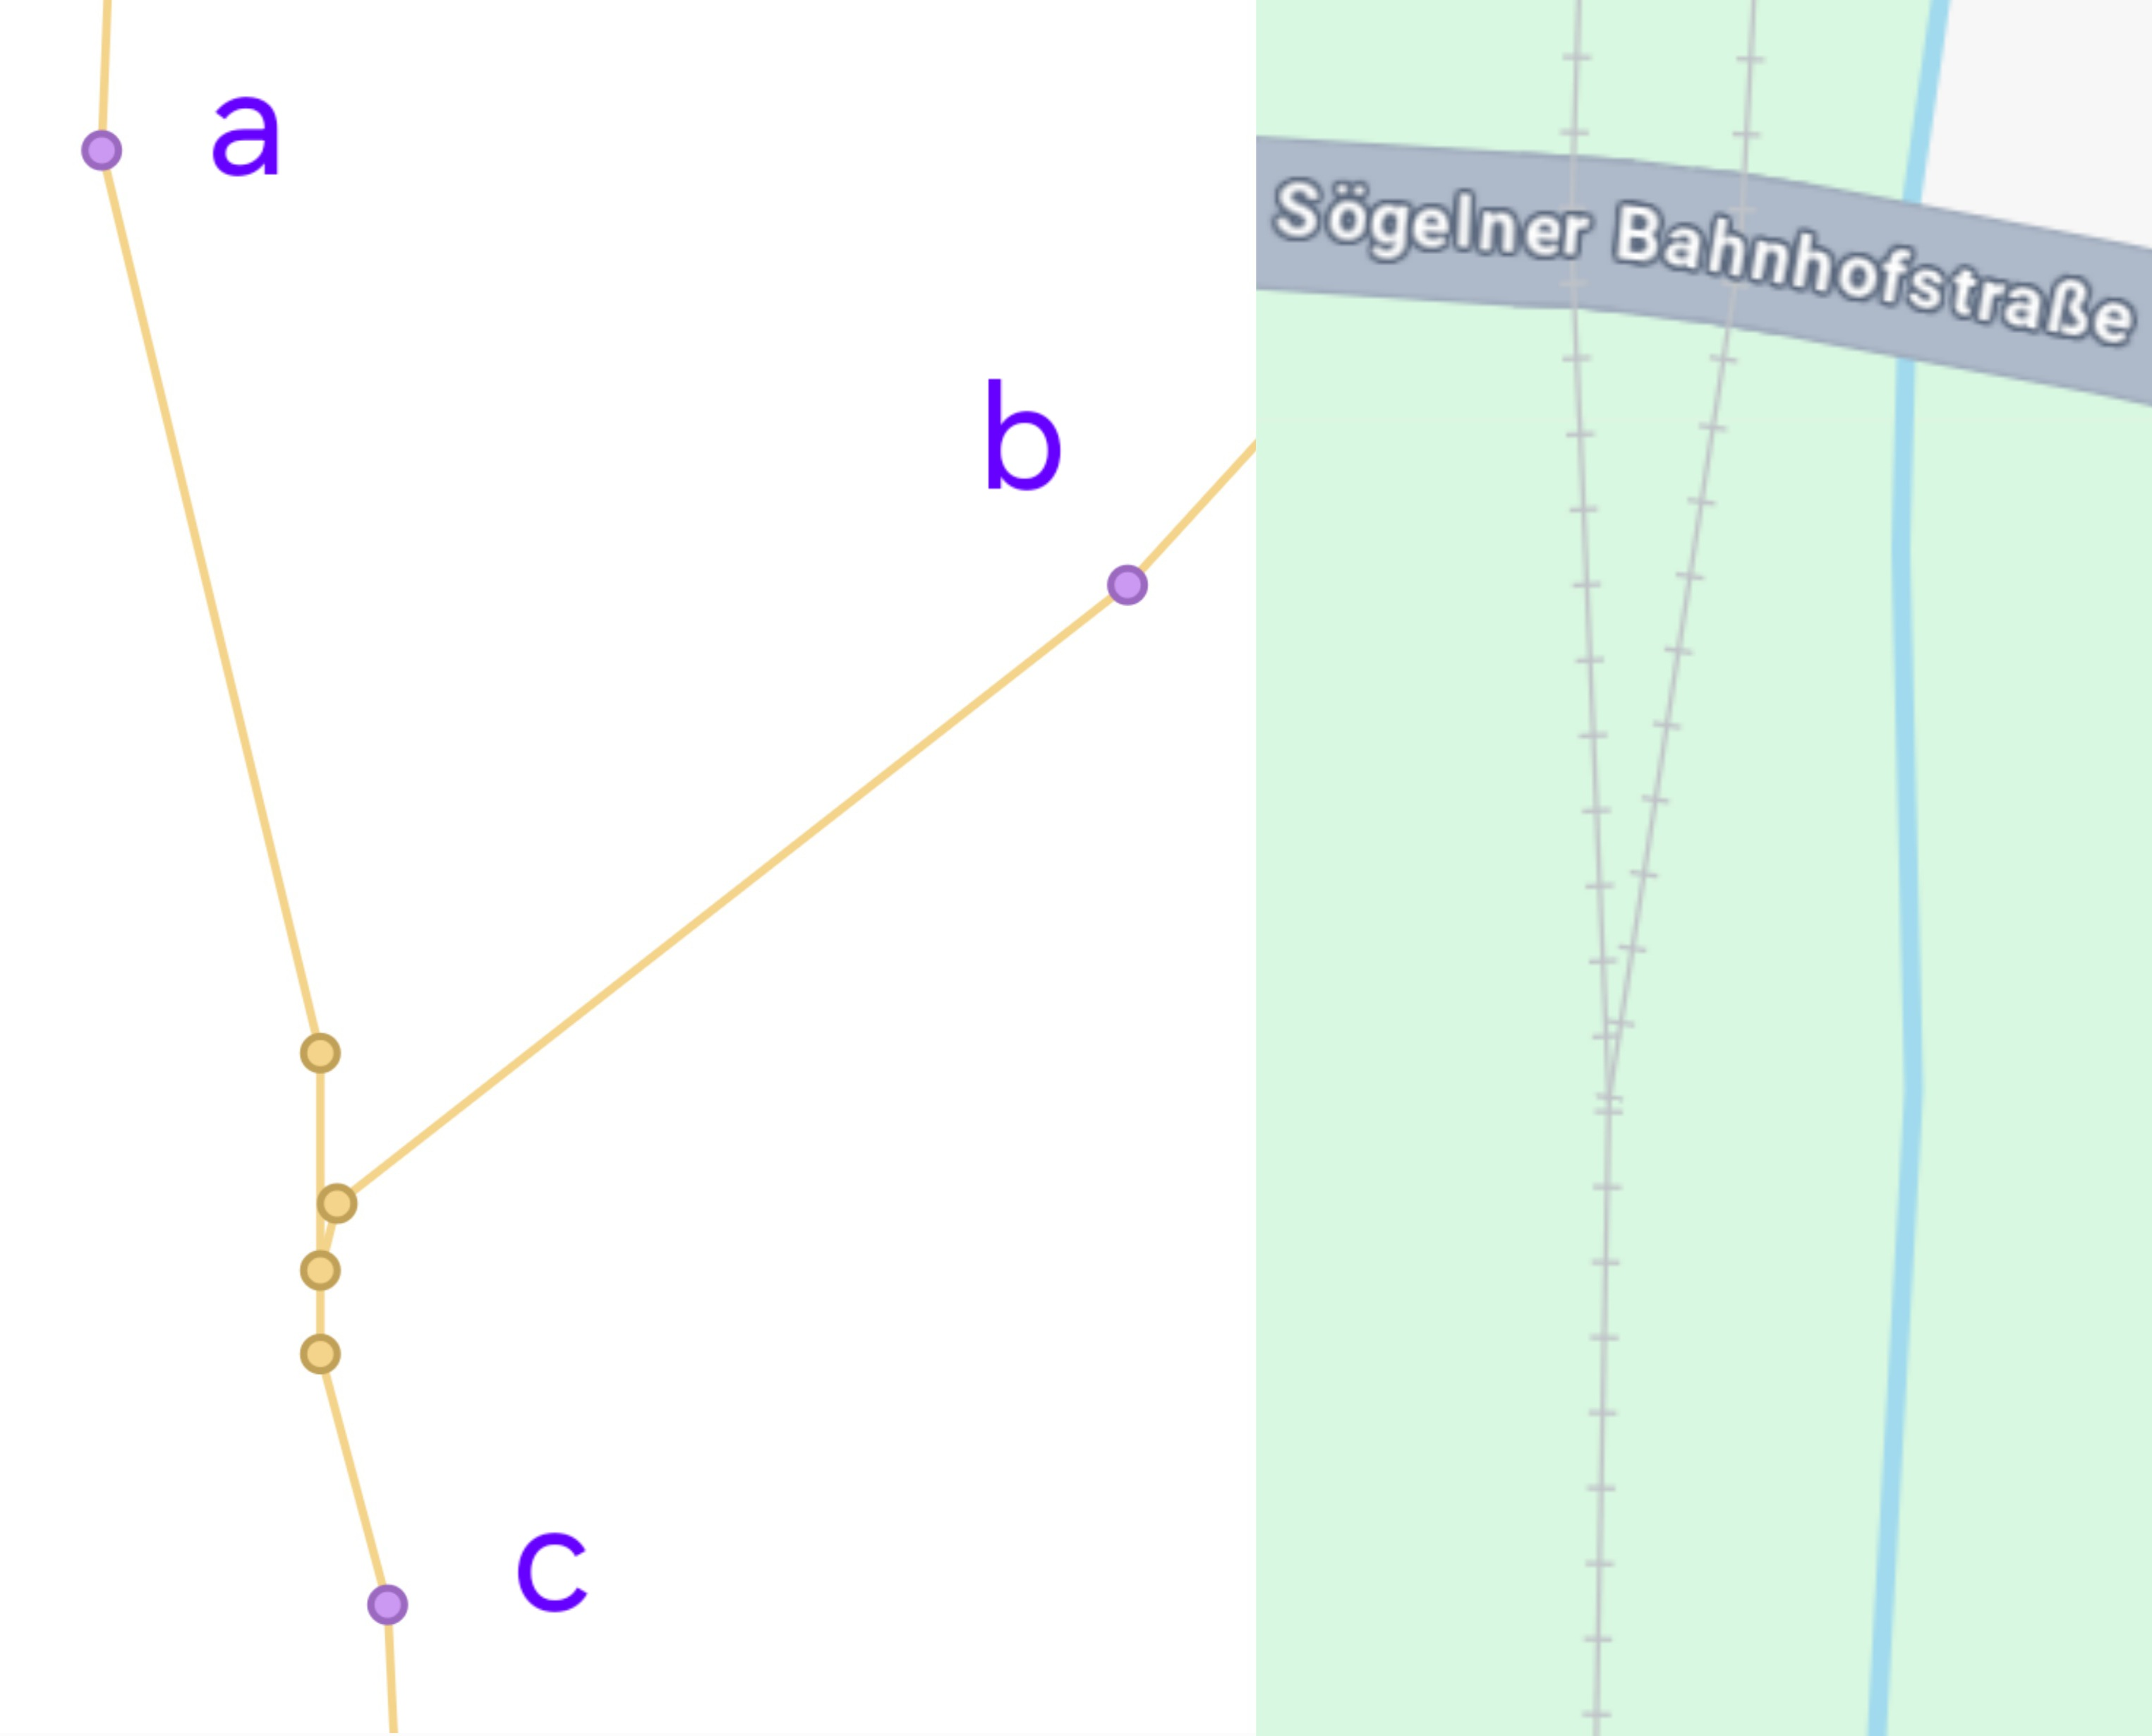
\includegraphics[width=\linewidth,keepaspectratio]{images/junction_example.jpg}
  \caption{German rail junction. a, b and c are $s$ nodes; on the right a Maps view.}
  \label{fig:junction}
\end{wrapfigure}
In the provided example, it is clear that in order to go from $a$ to $b$, one must pass through $c$, and, while in this case the connection is straightforward ($a \, - \, c$  ;  $b\, - \, c$) a lot of junctions are intertwined with each other and there are many edge cases.\\
Until the definition of \emph{path} is addressed properly, centrality measures of betweenness and closeness could be misleading.

The objective is therefore to prune the network as much as possible, using only non-spatial topological features, such as degree, while retaining all the useful information on how different stations are connected with each other\footnote{Note that in the pruning process, one could keep records of the distance between $ns$ nodes before removing them, and encode it in the edges of the pruned graph.}.
\\
\\
\\
\\
\\
\\

\section{Pruning algorithm, overview and visualization}
Upon data extraction, each linestring object is immediately reduced to just the first, second, second-last, and last points; then, a list of protected nodes is defined, its elements are:
\begin{itemize}
  \item $s$ nodes,
  \item neighbors of nodes $v$ s.t. $k_v \geq 3$ and $v$ does not belong in any $3-clique$, 
  \item all nodes that belong in a $3-clique$.
\end{itemize}
The choice of protecting neighbors of high-degree nodes is an attempt to preserve the spatial information that would be needed to decide which paths are allowed through a junction, this can be achieved simply by forbidding the path between the nodes that form the lowest angle with that junction (although it is not that easy for 4 or 5 way junctions). The focus on 3-cliques is motivated by the fact that those types of junction always connect everyone with everyone else, without needing spatial information.\\
The algorithm itself first removes non protected degree-1 (dangling) nodes, than all non protected degree-2 nodes, then, intermediate nodes between almost-3-cliques are removed. \\
Throughout the process, an interactive visualization tool was used; here is a 
\href{https://ale-neri-137.github.io/PoCN_project/french_rail_before.html}{before} and 
\href{https://ale-neri-137.github.io/PoCN_project/french_rail_after.html}{after} example for the French rail network.

 




\newpage
